% Michal Kovac's master thesis
%
\documentclass{article}

\author{Michal Kov\'{a}\v{c}}
\title{User oriented language for powerful data mining with Ferda}
\date{\today}

\begin{document}
\section{Introduction}
\subsection{History}
GUHA method

LISp-Miner

Michal Kov\'{a}\v{c}, Tom\'{a}\v{s} Kucha\v{r}, Alexander Kuzmin and Martin Ralbovsk\'{y} have started to work on the Ferda Data Miner in the year 2003. The project lead was Jan Rauch. The basic aim of this project had to be creating of a user friendly user interface for the LISp-Miner project. It was achieved, but the Ferda was created in mind of future extensions and main parts of the application are independend ondata mining at all.

Ferda is user orieted application for working with special objects called boxes. Boxes have sockets and a user can connect to these sockets another boxes. Boxes have functions, sockets are places for parameters for these functions. The Ferda Data Miner is Ferda with boxes for data mining.

First boxes for data mining were written for LISp-Miner generators. It was hardly extensible. Later Tom\'{a}\v{s} Kucha\v{r} as part of his diploma thesis written own implementation of basic GUHA procedures for the Ferda Data Miner.

There are many new boxes created for special applications like decission trees, ontology mapping or relational data mining.

\section{Ferda Data Miner}
\subsection{Implementation}

Base parts of Ferda has been written in C\# 2.0. Ferda runs on both .NET Framework and Mono. Some parts of new boxes use also Java platform. Ferda uses middleware Internet Communications Engine for communication between its parts. Every part can be written in another language and run on another computer. For easier developement many third party libraries and application have been used, for mainly NAnt, NUnit, NDoc, Netron Graphic Library and DockDotNet. 

Ferda is under second version of General Public License. It allow everybody to use it for free, redistibute it, change the code the code the result will be still under the General Public License.

Aim was to create application which is internationalized, well documented, modular, user friendly and conforms microsoft standards.

Ferda is client-server application. Client executable is FerdaFrontEnd.exe and we call that part FrontEnd. There isn't one server executable instead there are more separate modules which all can act as separate application. FrontEnd comunicates with all of them. Some of these modules implements boxes so we call them box modules, other are helper modules like GUHA mining engine.

\pgfuseimage{designimage}

FrontEnd uses assembly FerdaModulesManager.dll for communicating with modules. This assembly is layer of abstraction so that FrontEnd soes not know that modules are not implemented local.

Another assembly that is used by FrontEnd is FerdaProjectManager.dll. It obhospodaruje projects. Project consists of box instances which are placed in an archive and views. Views adds to boxes its placement on a desktop. This manaher is able to load project from xml file and save it to xml file.

FrontEnd also loads add ins. Add ins can extend functionality of FrontEnd in many ways. Mainly it is used for modules for interaction and setting modeles. Modules for interaction work on top of some box module. It for example show results of functions returned by the box module. Setting modules are used for helping with setting nonstandard properties.
8
Comunucation between FrontEnd and modules and between modules itself are done be Internet Commu6nication Engine (ICE). ICE is strong modern middleware. Thanks to usage of ICE Ferda is language and framework independend and it allow as to run different modules on different computers, but it doesn't add big complexity to the application. It an be also used for distributed computing.

IceGrid applications, which manage available modules and load them on demand, runs on a network. Modules manager use these application for getting modules.

Every box module implementation has it's factory class. This factory class creates box module instances. There is one more layer -- every box module factory has it's factory class, we call it box module factory creator. It is used as singleton.

\pgfuseimage{creatorFactoryimage}

FrontEnd asks box module factory creator for creation of only one box module factory for one box class. Creator has methods independend on both instance of box module and FrontEnd connected and factory has methods independend on box modules, but dependend on FrontEnd (for example localized names of properties). When FrontEnd is not connected for longer time all factory instances and box module instances are destroyed.

Box modules mainly consists of sockets, properties and functions. Sockets are places where you can connect another box module. They are parameters for functionality of the box module. Properties are also parameters and can be viewed as socket, but can be configured both by connecting a box to the socket and by setting the property in the property grid.

Functions is some class which box returns. This class represents the functionality of the box.

Box module has also identifier, icon, svg design, names of categories, box modules asking for creation, actions, name of property driving label and dynamic help.

\subsection{Ferda as programming language}
The main concept of Ferda is to be functional language. Basic view is that a box is a function and sockets are properties of that function. There is no need to talk about properties, because properties are also usable by sockets. To be more precise, box can be not only viewed as one function, but as set of functions. As was writen box returns class as functions. So every method of such class can be viewed as separate function. Box can also return diferrent functions class depending on its parameters. 

Box is $\left<S,F\right>$ where
\begin{itemize}
	\item $S$ is a set of sockets
	\item $F$ is a set of functions
\end{itemize}
	
Socket is $\left<n,T\right>$ where
\begin{itemize}
	\item $n$ is socket name
	\item $T$ is a set of box types
\end{itemize}

We have prediate $has(f,i)$ where $f$ is function and $i$ is ``Ice identifier''

Type is $\left<i,S\right>$ where
\begin{itemize}
	\item $i$ is ``Ice identifier''
	\item $S$ is a set of $\left<n,i\right>$
	\begin{itemize}
		\item $n$ is socket name
		\item $i$ is ``Ice identifier''
	\end{itemize}
\end{itemize}

Box $B=\left<S,F\right>$ is of type $A=\left<i,Z\right>$ iff 
\begin{enumerate}
	\item $(\forall \left<n,j\right>\in Z)(\exists \left<m,T\right>\in S)(\exists \left<y,W\right>\in T)(m=n \wedge j=y)$
	\item $(\exists f\in F)(has(f,i))$
\end{enumerate}
	
\begin{itemize}
	\item Box consists of functions
	\item Sockets are parameters of these functions
	\item Property is also socket
		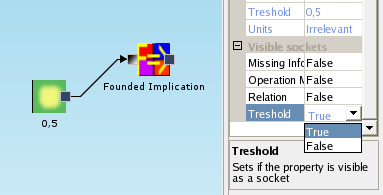
\includegraphics[width=7cm]{property_as_socket}
\end{itemize}

	\begin{block}{What is missing?}
		\begin{itemize}[<+->]
			\item Moving work from one project to another
			\item Basic math boxes
			\item Recursion
			\item Other language boxes
			\item Ferda specific language boxes
			\item Data mining specific boxes for user programming
		\end{itemize}
	\end{block}

\section{Lambda calculus}
Base of functional languages in in lambda calculus. 

%rekurzivne spocetny
%vsecno je funkce
%typovany/netypovany
\section{Functional languages}
%prvky - vzhledem k Ferdovi
%jak delaji rekurzi / lambdu - rozsil mezi structuralnim a funkcionalnim jazykem

\section{Making things better in actual implementation}
result browser - aby umel heterogenni vysledky - vystup z 4FT + vystup z CF

Implementation of GUHA in Ferda by 'small' boxes.
\section{Lambda expression}
\section{Sequences}
\section{Examples}
\subsection{Four fold task in recursion}
\subsection{Getting basic information from table}
\section{Implementation details}
\section{Problems in Ferda code}
\section{Future tasks to do in ferda}
%popis jednotlivych tasku s narocnosti, uzitkem - bodove ohodnotit

% modules for interacion je treba vylepsit
\end{document}
